\documentclass[]{beamer}

\input{settings/special_beamer}
\usepackage[T2A]{fontenc}
\usepackage[utf8]{inputenc}
\usepackage[english, russian]{babel}
\usepackage{hyperref}     % ТАК_НУЖНО
\hypersetup{unicode=true} % ТАК_НУЖНО
\usepackage{amsmath}
\usepackage{amssymb,textcomp, esvect,esint}
\usepackage{amsfonts}
\usepackage{amsthm}
\usepackage{graphicx}
\usepackage{indentfirst}
\usepackage{xcolor}
% \usepackage{enumitem} %--- ломал нумерацию!?

\usepackage{graphicx}
\usepackage{booktabs}
\usepackage{caption}
\usepackage{listings}
\usepackage{tikz}
\usepackage{xcolor}
\usepackage{cancel}


\usepackage[justification=justified]{caption}

% \usepackage{media9}
% \usepackage{animate}
% \usepackage{threeparttable}
% \usepackage{pifont}


\usepackage{import}
\usepackage{xifthen}
\usepackage{pdfpages}
\usepackage{transparent}

% \usepackage{natbib}

\usepackage[skip=1pt]{caption}

\usepackage{ifthen}
\definecolor{darkgreen}{RGB}{10,90,10}
\definecolor{crane}{RGB}{255,187,3}
\definecolor{seahorse}{RGB}{215,211,233}

% \usetikzlibrary{tikzmark,fit,shapes.geometric} % рисование кружочков


\usepackage{subfigure}

\newcommand{\kB}{k_{\textnormal{B}}}
\newcommand{\vcap}{\sub{v}{c}}
\newcommand{\dC}{\,{}^\circ\textnormal{С}}


\newcommand{\incfig}[1]{%
    % \def\svgwidth{\columnwidth}
    \import{figures/}{#1.pdf_tex}
}

% \usepackage{circuitikz}

\newcommand{\vc}[1]{\mbox{\boldmath $#1$}}
\newcommand{\smallvc}[1]{\scalebox{0.65}{\mbox{\boldmath $#1$}}}

\newcommand{\T}{^{\text{T}}}
\newcommand{\R}{\text{R}}
\newcommand{\const}{\text{const}}
\newcommand{\sub}[2]{#1_{\textnormal{#2}}}
% \renewcommand{\tg}{\mathop{\mathrm{tg}}\nolimits}

\renewcommand{\Im}{\mathop{\mathrm{Im}}\nolimits}
\renewcommand{\Re}{\mathop{\mathrm{Re}}\nolimits}
\renewcommand{\d}{\, d}
\renewcommand{\leq}{\leqslant}
\renewcommand{\geq}{\geqslant}

\newcommand{\cmark}{\text{\ding{51}}}
\newcommand{\xmark}{\text{\ding{55}}}



\definecolor{mygray}{gray}{0.6}
\definecolor{mygreen}{RGB}{8,99,44}
\definecolor{myred}{RGB}{164,0,0}



\newcommand{\iitem}[1]{\item[\textcolor{myred}{\scalebox{0.7}{$\blacksquare$}}]{#1}}
\title[Оптимизация в МОЛ]{Оптимизация количества атомов тулия в
магнитооптической ловушке}


\author{Хоружий Кирилл}
\institute[РКЦ, МФТИ]


\let\tg\undefined %костыль связанный с русским языком и tg

\setbeamertemplate{caption}[numbered]

\begin{document}
\maketitle


\frame{
	\input{slides/1} \frametitle{Construction}
}

\frame{ %установка
	\only<1>{
\begin{figure}[h]
        \centering
        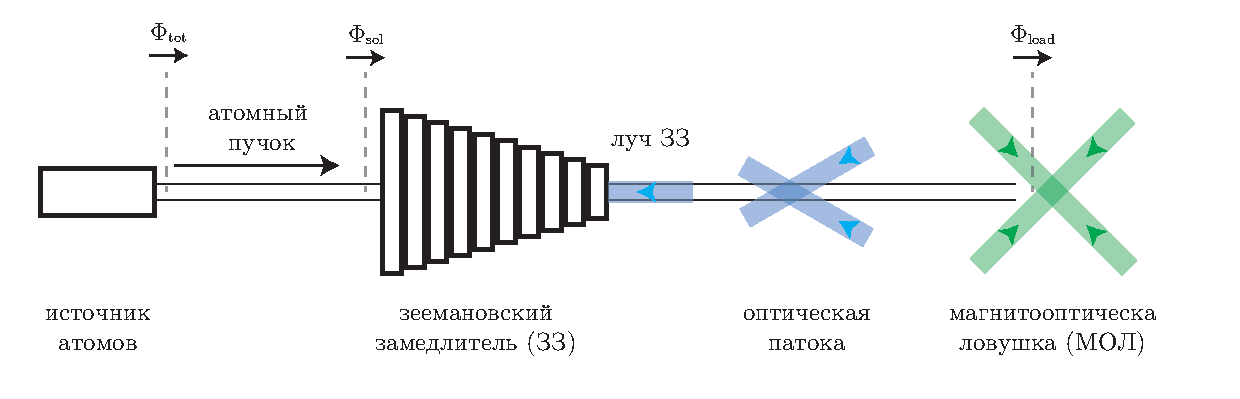
\includegraphics[width=0.68\textwidth]{../MOT/figs/sheme.pdf}
        \caption{Принципиальная схема установки}
    \end{figure}

    \begin{figure}[h]
        \centering
        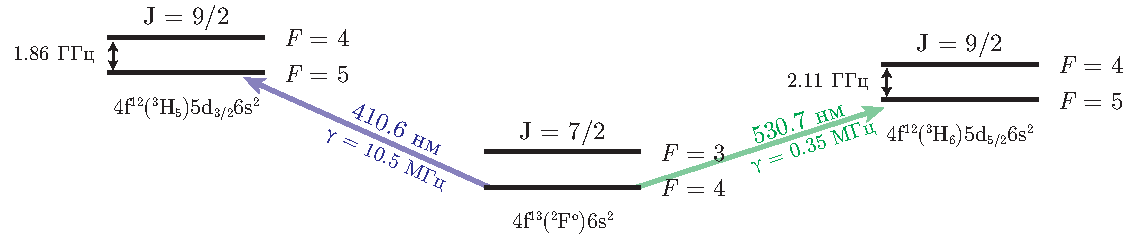
\includegraphics[width=0.68\textwidth]{../MOT/figs/tm_pres.pdf}
        \caption{Используемые в эксперименте атомные переходы}
    \end{figure}
}

\only<2>{
\begin{minipage}{0.68\textwidth}
    \begin{figure}[h]
        \centering
        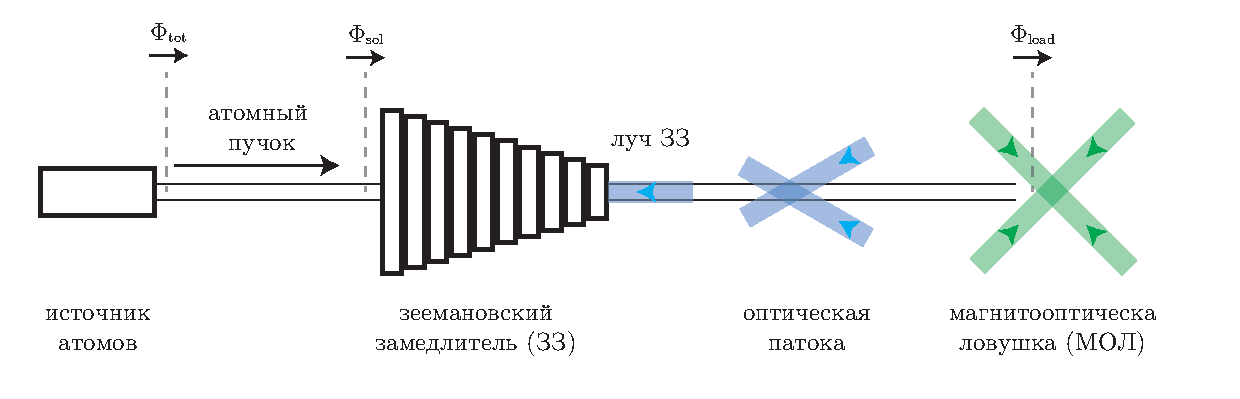
\includegraphics[width=1.0\textwidth]{../MOT/figs/sheme.pdf}
        \caption{Принципиальная схема установки}
    \end{figure}

    \begin{figure}[h]
        \centering
        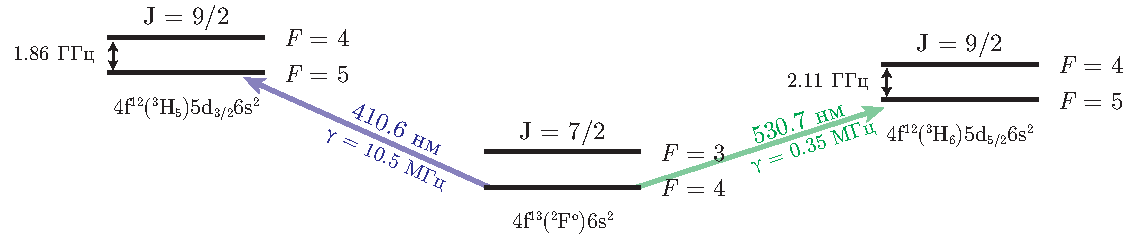
\includegraphics[width=1.0\textwidth]{../MOT/figs/tm_pres.pdf}
        \caption{Используемые в эксперименте атомные переходы}
    \end{figure}
\end{minipage}
\hfill
\begin{minipage}{0.31\textwidth}

$\sub{t}{life}$ -- время непрерывной \\ работы установки

\phantom{42}


Ограничения на $\sub{t}{life}$:
\begin{itemize}
    \iitem{заканчиваются атомы}
    \iitem{напыление на зеркало перед замедлителем}
\end{itemize}

\phantom{42}

\textbf{Задача}: \\ увеличить $\sub{t}{life}$, сохранив $\sub{\Phi}{load}$


\end{minipage}
}
\only<3>{
\begin{minipage}{0.68\textwidth}
    \begin{figure}[h]
        \centering
        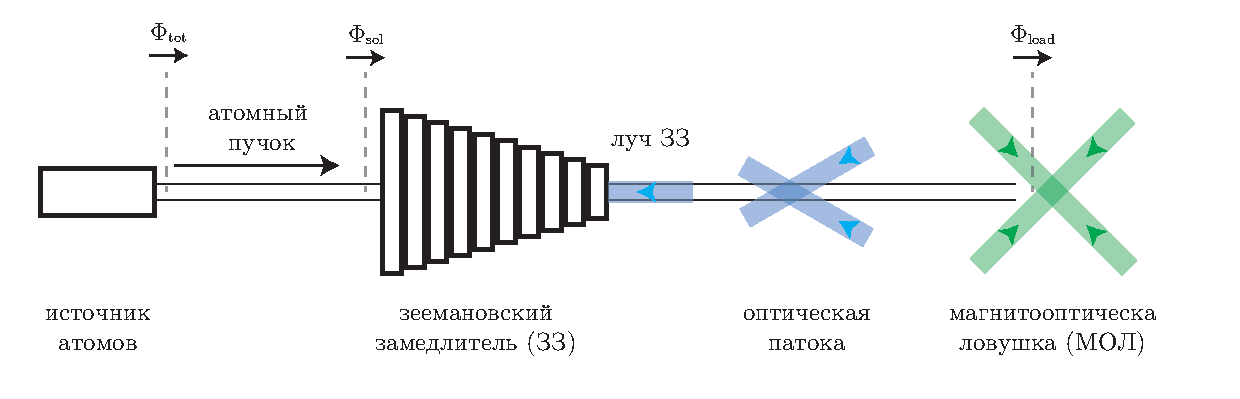
\includegraphics[width=1.0\textwidth]{../MOT/figs/sheme.pdf}
        \caption{Принципиальная схема установки}
    \end{figure}

    \begin{figure}[h]
        \centering
        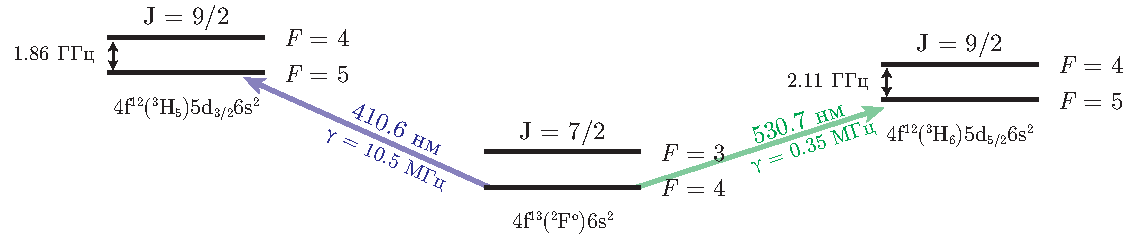
\includegraphics[width=1.0\textwidth]{../MOT/figs/tm_pres.pdf}
        \caption{Используемые в эксперименте атомные переходы}
    \end{figure}
\end{minipage}
\hfill
\begin{minipage}{0.31\textwidth}
\textbf{Задача}: \\ увеличить $\sub{t}{life}$, сохранив $\sub{\Phi}{load}$

\begin{align*}
    \sub{t}{life} &\propto 1/\sub{\Phi}{tot}(T) \\    
    \sub{\Phi}{sol} &\propto \, \sub{\Phi}{tot} \\ 
    \sub{\Phi}{load} &= \eta\, \sub{\Phi}{sol}
\end{align*}

$\eta$ -- эффективность ЗЗ

\phantom{42}


Дальнейшие действия:
\begin{itemize}
    \iitem{понижение $T$}
    \iitem{ повышение $\eta$}
\end{itemize}

\end{minipage}
}
   


 \frametitle{Общая схема охлаждения}
}


\end{document}



